\chapter{Estado del arte}

En este capítulo estudiaremos y analizaremos los diferentes enfoques dados históricamente para nuestras tareas, \textbf{clasificación de tumores cerebrales} y \textbf{la segmentación de tumores cerebrales}. Abordando desde el inicio del estudio del problema pasando por la explosión de métodos basados en Aprendizaje profundo con la constitución de \textbf{BraTS} hasta nuestros días. Se pondrá especial énfasis a las soluciones actuales comparándolas desde sus diferencias en metodología y perspectiva.

Por un lado, la clasificación entre los dos tipos de tumores no es tan relevante a la hora de diseñar un sistema de ayuda a la toma de decisión ya que clínicamente sí existe una característica diferencial entre ambos, su \textbf{localización}. Los meningiomas aparecen entre el cráneo y el cerebro no internamente en el cerebro como los glioblastomas. Esto hace que un médico pueda distinguirlos sin requerir una gran asistencia para la mayoría de los casos. No obstante, la clasificación puede ayudar a la toma de decisiones en el tratamiento ya que debido a la naturaleza difusa de los glioblastomas estos pueden aparecer en la misma localización que algunos meningiomas y pueden ser confundidos. Sin embargo, la clasificación entre tipos de tumores no es el elemento crítico para la supervivencia del paciente que depende de la eliminación del tumor donde su segmentación toma un papel crucial. Por esto, veremos como el estado del arte del problema de segmentación es mucho mayor que el del problema de clasificación.

Por otro lado, la tarea de predicción de la evolución del tumor debido a la baja densidad de instancias temporales de los datos existentes hacen que este problema no sea tratado en trabajos. No hemos encontrado literatura al respecto. 

Los grandes esfuerzos se han realizado en entorno a la segmentación, ya que otras tareas que conforman su diagnóstico se verían arrastradas.

\section{Revisión histórica de clasificación binaria de tumores}

Dentro de los problemas de clasificación que se pueden plantear para caracterizar a los tumores cerebrales se pueden encontrar clasificación multi-clase para diferenciar entre tipos de tumores (glioblastomas, meningiomas u otros tumores más raros y menos frecuentes) o clasificación multi-grado (low- or high- grade) para caracterizar el estado de avance del tumor.

En este trabajo solo nos centraremos en clasificación multi-clase para los dos tipos de tumores más frecuentes y de los que disponemos de etiquetas por BraTS, glioblastomas y meningiomas.

A continuación, se pretende recoger los trabajos más relevantes realizados entorno a esta clasificación multi-clase ordenados en el tiempo, haciendo especialmente hincapié en las soluciones basadas en aprendizaje profundo. 

\section{Revisión histórica de segmentación}

Diferentes dificultades han sido las que a pesar de años de desarrollo aún encontrar un algoritmo para la segmentación de tumores cerebrales sea algo mejorable. 

\begin{enumerate}
	\item \textbf{Incertidumbre en la localización} : Como vimos no existe una zona concreta en general para la aparición de los tumores cerebrales. A excepción, de los meningiomas localizados en zonas superficiales del cerebro y aún siendo una región muy amplia, incluso ya desarrollado un tumor pueden aparecer otros localizados en regiones muy distintas de la original. 
	\item \textbf{Incertidumbre en la morfología} : A diferencia de otras patologías, cada tumor cerebral presenta un tamaño y forma completamente distintas y donde en principio no se puede apreciar un patrón distintivo. Esto hace que sea muy complicado y generalmente aporte malos resultados, la construcción de sistemas basados reglas u otras aproximaciones que no incluyen una componente de aprendizaje.
	
	\item \textbf{Bajo contraste} : Una buena resolución y contraste son características muy importantes para entender la información de una imagen. Las imágenes IRM producidas en una resonancia debido a proyecciones de imagen y procesos de tomografía usualmente ofrecen una baja resolución y contraste haciendo más difícil la definición de bordes entre diferentes tejidos de la imagen. Una segmentación precisa es difícil de conseguir.
	
	\item \textbf{Sesgo en las etiquetas}. Existen indicios para pensar que las etiquetas proporcionadas pueden presentar ruido. El proceso de segmentado por parte del personal médico 
	depende de su experiencia profesional lo cual puede llevar a cometer errores. Por ejemplo, se han presentado eventualmente discrepancias entre distintos anotadores: algunos tienden a conectar todas las pequeñas regiones de un tejido mientras que otros las segmentan de forma más precisa y separada. 
	
	\item \textbf{Desbalanceo en el tejido} : Dentro de la segmentación entre los diferentes tipos de tejidos, usualmente existe un el tejido enfermo y que compone la lesión tumoral es usualmente más pequeño que el tejido sano. Esto podría afectar en el proceso de aprendizaje creando rechazo a identificar al tejido enfermo. 
	
	\item \textbf{Desbalanceo entre pacientes} : En el conjunto de datos tenemos muchos pacientes de norteamerica y de ascendencia blanca, pero pocos de otros origenes como el africano. Además, de tener un sesgo claro de edad ya que existen pocos casos en niños. Esta falta de datos puede impedir que exista una buena generalización para estos casos más aislados.
	
\end{enumerate}


	A continuación, se presenta una revisión histórica sobre la segmentación de tumores cerebrales hasta 2021 apoyada en \cite{liu2023deep}. Se presenta una línea del tiempo con los principales trabajos de estudio.
	
	\begin{figure}[H]
		\centering
		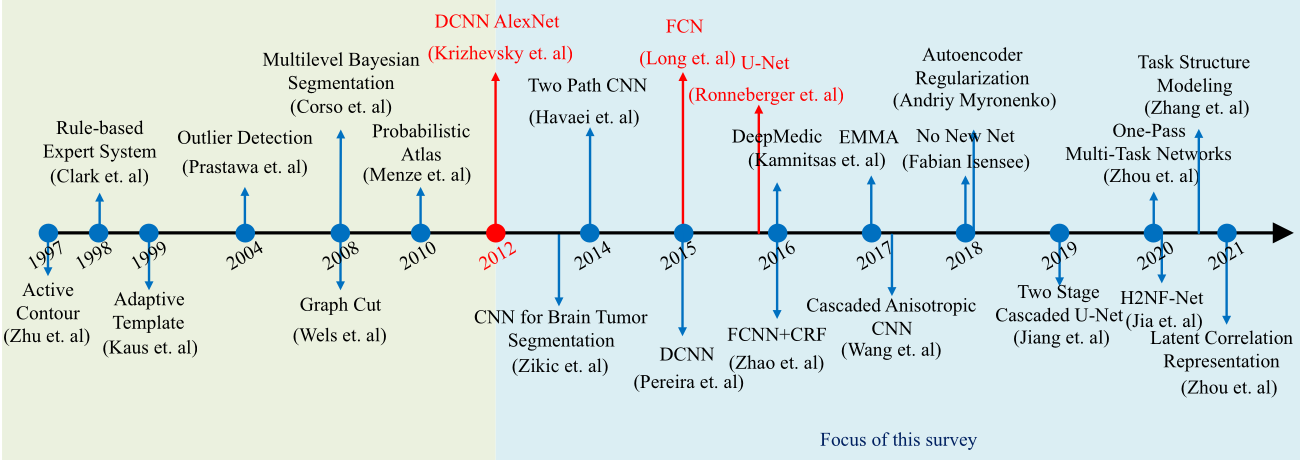
\includegraphics[width=1.0\linewidth]{imagenes/evolution_stateofart.png}
		\caption{Evolución histórica del estado del arte hasta 2021.}
	\end{figure}
	
	En la década de 1990 investigadores como \cite{zhu1997computerized} fueron pioneros al utilizar una red Hopfield con un modelo de contornos activos para extraer los bordes del tumor. Sin embargo, incluso el entrenamiento de una pequeña red como esta era algo computacionalmente costoso por las limitaciones de la época.  Desde 1990 hasta 2012, los métodos que iban surgiendo para la segmentación de tumores cerebrales estaban basados en métodos clásicos de aprendizaje con características extraídas a mano, sistemas expertos que se apoyaban en los histogramas de la imagen, plantillas para la segmentación y modelos gráficos. 
	
	A pesar de ser un gran paso inicial, tenían grandes deficiencias. Por ejemplo, la mayoría de ellos sólo se centraba en la segmentación de todo el tumor lo cual lleva a un modelo poco útil. Por otro lado, en los modelos basados en características extraídas se hacía muy tedioso poder usarlos eficazmente ya que este paso de extracción dependía de conocimiento previo experto que en ningún momento se pudo llegar a representar en un modelo. En último lugar, los mismos problemas que compartimos hoy en día sobre el desbalanceo y la incertidumbre del problema eran mucho más agresivos. 
	
	Tras 2012 con la revolución del Deep Learning, se introducen nuevas tecnologías (Redes neuronales convolucionales y U-net) que mejorarán los resultados obtenidos hasta el momento. 
	Se empezarán a construir arquitecturas encoder-decorder convolucionales para conseguir pipelines completos para la segmentación. El aprendizaje profundo toma el problema de lleno proclamándose el enfoque que define el estado del arte.
	
	Podemos clasificar las soluciones basadas en aprendizaje profundo aportadas en tres categorías según el principal problema para que el están pesadas. Sin embargo, como veremos en las soluciones más actuales lo ideal es tratar con los tres problemas.
	
	\subsection{Métodos que se enfocan en la arquitectura}
		
		 Para poder obtener redes que automáticamente extraen características discriminativas a altas dimensiones es necesario un efectivo diseño de módulos y arquitecturas. Por un lado, se pretende que la arquitectura sea capaz de aprender las características distintivas de los tejidos y a localizar regiones de interés por medio de añadir profundidad a la red, a través de mecanismos de atención o la fusión de características entre las resonancias. Por otro lado, se pretende minimizar la cantidad de parámetros entrenables de la red o conseguir un entrenamiento más rápido.
		 
		\subsubsection{Diseño de bloques especializados}
			
			Los primeros trabajos que tenían este objetivo comenzaron por basarse en arquitecturas bien conocidas como AlexNet o VGGNet a través del uso de una única imagen de la resonancia completa como entrada de la red.
			
			Para la mejora de resultados, se optó por introducir todas la secuencia de imágenes de una resonancia como entrada de la red y añadir más capas convolucionales. Con ello, teníamos redes más profundas pero que pronto empezaban a sufrir los problemas de la explosión y desvanecimiento del gradiente durante el proceso de entrenamiento. Para ayudar a lidiar con estos problemas, se introdujo a las redes, \textbf{conexiones residuales} \cite{chang2016fully}. Conectando la entrada de la red con su salida, convergiendo más rápido y con mejores resultados. 
			
			Este proceso de aumento de profundidad con conexiones residuales no sería definitivo porque también conlleva el sacrificio de resolución espacial. Se reemplazaría en trabajos siguientes, el uso de la convolución simple por convoluciones dilatadas. El \textbf{uso de convoluciones dilatadas} traería el aumento del espacio receptivo (ya que se aplica una convolución a un espacio mayor de la imagen) sin necesidad de introducir parámetros a la red. La convolución dilatada se vería especialmente útil por ejemplo en la segmentación de áreas grandes como suele ocupar el tejido ED (edema tumoral). 
			
			Respecto conseguir una buena eficiencia en tiempo de entrenamiento es conocido aplicar un reordenamiento en memoria de las imágenes de la resonancia similares (p. ej. el mismo slice en las 4 pruebas) de forma que se reduzcan la comunicación entrada-salida con GPU. Adicionalmente, autores como \cite{brugger2019partially} utilizan \textbf{conexiones reversibles}  en la red de forma que durante el proceso de backpropagation (backward pass) no se necesite memoria adicional para guardar las activaciones intermedias. Por último, para ahorrar en eficiencia se sustituye la convolución standard por la combinación de \textbf{convoluciones separables}.
			
			\subsubsection{Diseño de arquitecturas efectivas}
			
			La mayoría de los trabajos de recorrido histórico se encasillan en alguno de los siguientes dos enfoques de arquitectura: \textbf{redes neuronales convolucionales} para extraer características de la imagen y clasificar los patches o píxeles de la imagen según las etiquetas de los tejidos posibles o \textbf{redes encoder-decoder} en las cuales se puede definir un pipeline completo convolucional sin la necesidad de la agregación de capas totalmente conectadas.
			
			\begin{enumerate}
					
				\item \textbf{Redes neuronales convolucionales de una/múltiples trayectorias}
					
				A diferencia de una red convolucional de una única trayectoria, las redes de trayectoria múltiples tienen la capacidad de extraer diversas características a diferentes escalas. Estas características se combinan para su posterior procesamiento, usualmente en capas totalmente conectadas, permitiendo a las redes aprender tanto características globales como locales. 
				
				\begin{figure}[H]
					\centering
					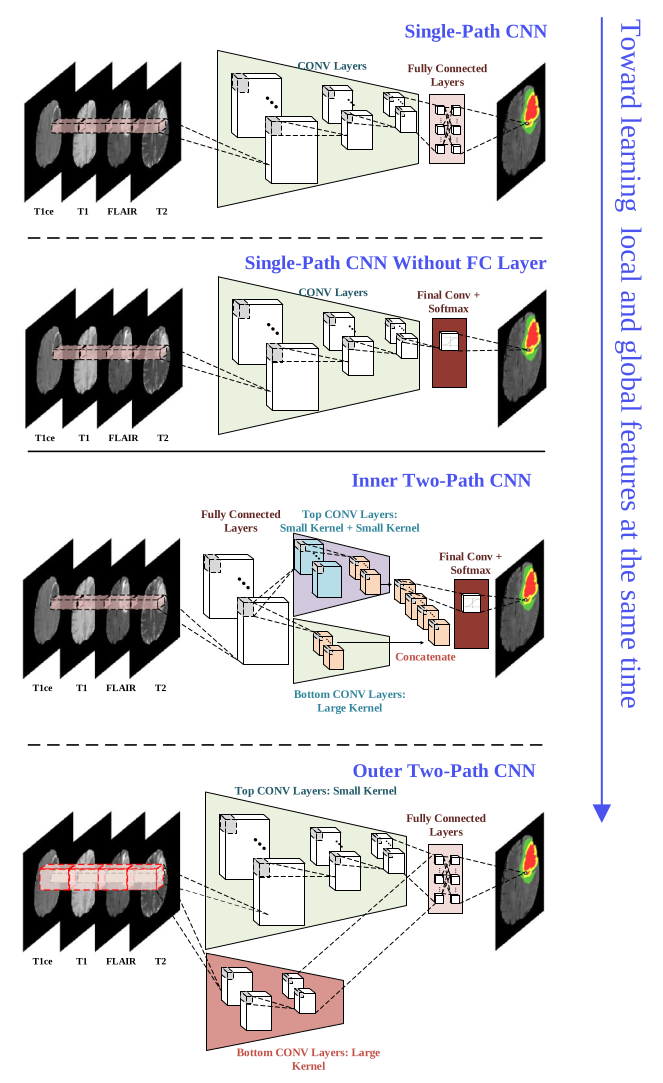
\includegraphics[width=0.5\linewidth]{imagenes/comparisonsinglemultipleCNN.png}
					\caption{Comparación entre arquitecturas de una y múltiples trayectorias. Imagen de \cite{liu2023deep}}
				\end{figure}
				
				Por ejemplo, \cite{havaei2017brain} desarrollaron una estructura de dos vías que integra información tanto local como global del tumor, utilizando núcleos de convolución de diferentes tamaños.
				
				\begin{figure}[H]
					\centering
					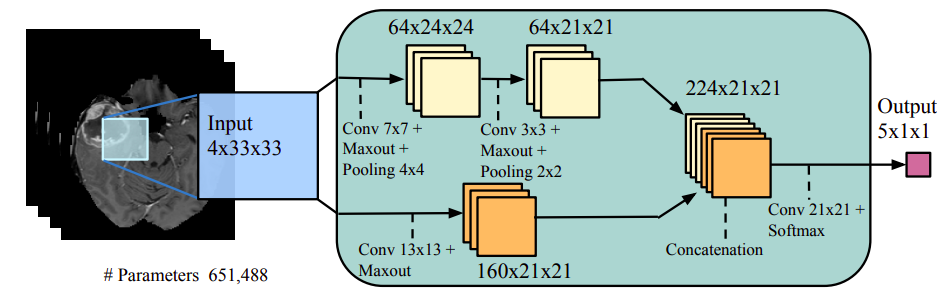
\includegraphics[width=0.75\linewidth]{imagenes/havaei2017architecture.png}
					\caption{Arquitectura de dos vías de \cite{havaei2017brain}}
				\end{figure}

				Otros enfoques, como el de \cite{kamnitsas2017efficient}, optan por aprender información global y local desde la entrada misma, utilizando redes de doble vía, patches de diferentes tamaños y pequeños núcleos de convolución. 
				
				Este tipo de arquitecturas fueron una de las primeras aproximaciones que empezaban adaptarse con éxito a las complejidades de la segmentación de tumores cerebrales. Sin embargo, veremos como la dificultad de un buen ajuste en el diseño de estas arquitecturas todavía seguía siendo un problema.
					
				\item \textbf{Arquitecturas Encoder-Decoder}
				
				Las redes de una/múltiples trayectorias toman como input un patch de una cierta región de la imagen y dan como output la clasificación del tejido que existe en ese patch. Este enfoque hace que obtener una buena arquitectura que haga la transformación de los patches a información categórica sea complicado por varios motivos: 
				\begin{enumerate}
					\item Existe una gran \textbf{dependencia} entre el tamaño y calidad de los patches, y los resultados que ofrecería la arquitectura.
					
					\item Toda la transformación de características visuales (aunque, reducidas) a información categórica estaría concentrada en las capas totalmente conectadas. Las capas totalmente conectadas de un tamaño razonables para una capacidad de memoria usualmente utilizada \textbf{no puede totalmente representar un espacio de características tan grande}.
					
					\item Si necesitamos tener distintas redes separadas, el proceso de ajuste de cada una de ellas es independiente. Esto lo podemos interpretar como un coste añadido en términos de \textbf{eficiencia}.
					
				\end{enumerate}
				
				Para superar estos problemas en los siguientes trabajos se empieza a utilizar \textbf{FCN Redes neuronales totalmente convolucionales} y \textbf{U-net} basadas en arquitecturas encoder-decorder, de forma que se establece un pipeline completo desde la imagen a la segmentación.
				
				Una de los tipos más importantes de FCN para este problema es U-net. U-net consiste en la creación de conexiones entre el encoder y el decoder. Permitiendo una vinculación directa en el proceso de reducción y ampliación de dimensionalidad. Estas conexiones reciben el nombre de \textbf{Skip Connections} y pueden ayudar a las capas del decoder a recuperar detalles visuales aprendidos en el encoder, llevando a una segmentación más precisa.
				
				\cite{isensee2018brain} utilizan una U-Net dándole aún más énfasis a la tarea de una segmentación utilizando una función de pérdida basada en la similaridad Dice.
				
				Similar a las skip connections antes mencionado, el uso de conexiones residuales  y skip connections permiten el paso de características de alto y bajo nivel para una mejor segmentación final.
				
				\begin{figure}[H]
					\centering
					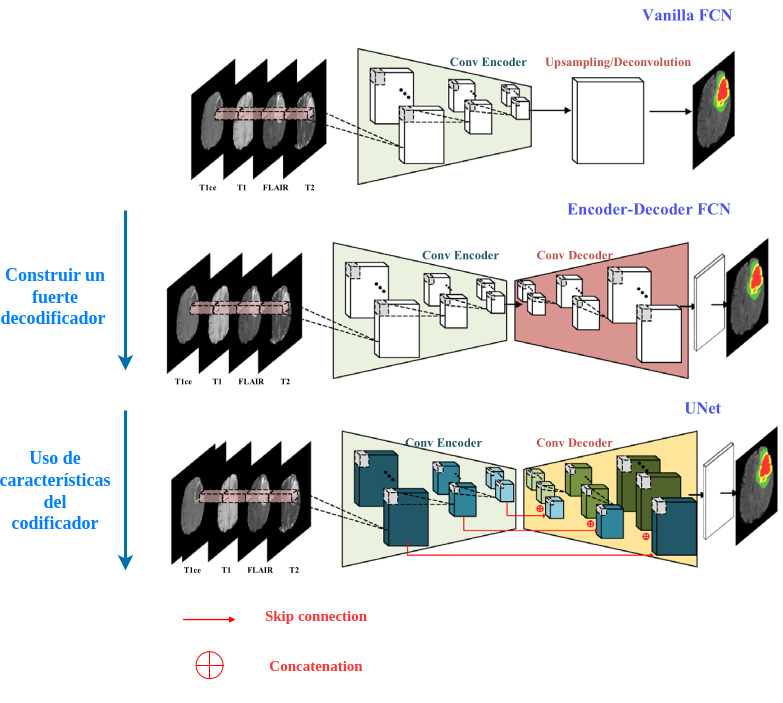
\includegraphics[width=0.85\linewidth]{imagenes/encoder-decoderIMG.drawio.png}
					\caption{Comparación de distintas arquitecturas encoder-decoder}
				\end{figure}
				
			\end{enumerate}
			
			
		\subsection{Métodos que tratan el desbalanceo}
		
		Como anunciábamos anteriormente el alto desbalanceo de los diferentes tejidos presentes en el cerebro de un paciente puede tener un impacto negativo en el proceso de entrenamiento. Motivados por métodos como los sistemas multi-expertos, se empezó a construir métodos específicos para este problema.
		
		Podemos diferenciar en:
		\begin{enumerate}
			\item \textbf{Diseños sobre la arquitectura}: Redes en cascada, ensamblado de modelos y arquitecturas multi-tarea.
			\item \textbf{Mejorar el entrenamiento}: Funciones de pérdida especializadas.
		\end{enumerate}
		
			\subsubsection{Redes en cascada}
			
			Una red en cascada es un conjunto de redes más pequeñas ordenadas en las cuales el output de la red anterior sirve como una input a la siguiente, formando una  <<cascada de redes>>. De esta forma, podemos tener redes especializadas en distintos niveles. 
			
			Las primeras redes de la cascada especializadas a características de más alto nivel y las siguientes de más bajo.
			
			Por ejemplo, en \cite{wang2018automatic} se utilizan tres redes especializadas para los tres regiones de tejidos definidas por BraTS. Empezando por la región más grande hasta la más pequeña. 
			
			Su primera red WNet segmenta a Whole Tumor, toda la lesión. La siguiente TNet segmenta al núcleo del tumor. Finalmente, Enet a la parte activa del tumor.
			
			
			\begin{figure}[!h]
				\centering
				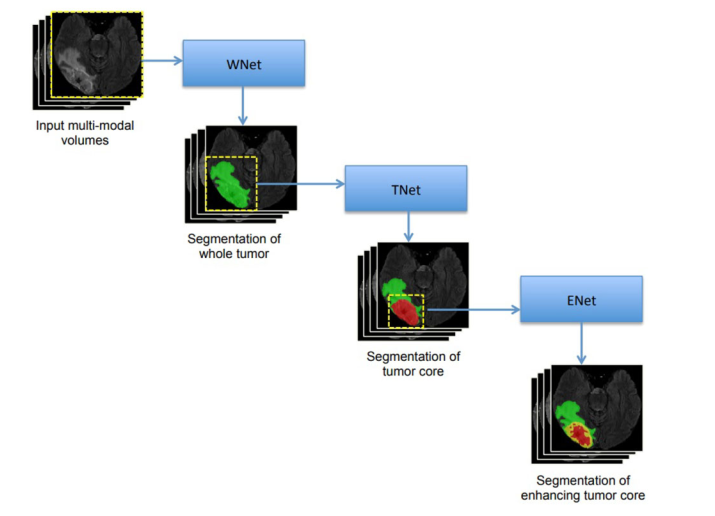
\includegraphics[width=0.5\linewidth]{imagenes/cascadestructure.png}
				\caption{Estructura de método en cascada de \cite{wang2018automatic}}
			\end{figure}
			
			La ventaja de este modelo es evitar la interferencia de las clases desbalanceadas, ya que cada red trata su clase como un problema de segmentación binaria. 
			
			Sin embargo, hace que la redes dependientes de otras dependan también de sus resultados. Si la primera red obtiene malos resultados, todas las siguientes redes se verán afectadas por ella.
					
			\subsubsection{Ensamblado de modelos}
			
			Una de las consecuencias que tiene el uso de una sola red es que está altamente influenciada por la elección de su hiperparámetros. Con el objetivo de obtener un más robusto y general modelo para la segmentación se puede combinar la salida de múltiples redes, ensamblarlas.
			
			El ensamblado de modelos aumentaría el espacio de hipótesis del modelo final evitando, la caída en óptimos locales debido a el desbalanceo de datos.
			
			EMMA  de \cite{kamnitsas2018ensembles} es uno de los primeros modelos para segmentación de tumores que es un ensamblado de varias redes. EMMA utiliza tres modelos: DeepMedic, una red FCN y una U-net para dar el output de los tres con una mayor confianza.
			
			\cite{jiang2020two} ganadores de BraTS2019 adoptaron una estrategia de ensamblado con $12$ modelos obteniendo entorno $0.6 - 1 \%$ mejores resultados que el mejor único modelo.
			
			\subsubsection{Arquitecturas multi-tarea}
			
			Todo lo descrito en esta revisión histórica gira entorno a la segmentación de tumores. Sin embargo, la desventaja que puede tener enfocarnos en esta sola tarea es que quizá los modelos específicos para segmentación ignoran información útil en las imágenes para otras tareas, que indirectamente pueda ayudar a obtener una mejor generalización en la segmentación de tumores. 
			
			Por un lado, esta idea radica en la suposición de que los modelos que aprenden más tareas están aumentando su aprendizaje en el dominio del problema y esto debería ser beneficioso para todas las tareas. Por otro lado, de una forma más justificada, sabemos que nos enfrentamos a cierto ruido que desconocemos en los datos y etiquetas por tanto si entrenamos para múltiples tareas en conjunto el modelo aprende representaciones más generales reduciendo el riesgo de sobreajuste. Añadir tareas a la arquitectura y aprenderlas en conjunto podría tener \textbf{un efecto regularizador}.
			
			Un claro ejemplo de esto es \cite{myronenko20193d} que usa como tarea complementaria la reconstrucción de la resonancia de entrada mediante un autoencoder. Teniendo un efecto regularizador sobre los parámetros compartidos del encoder que a diferencia de regularizaciones L1 o L2 que explícitamente añaden una penalización para evitar el sobreajuste, la tarea nueva añade una penalización en la dirección en la que ambas tareas son optimizadas reduciendo el espacio de búsqueda de los parámetros entrenables de la red.
			
			\begin{figure}[H]
				\centering
				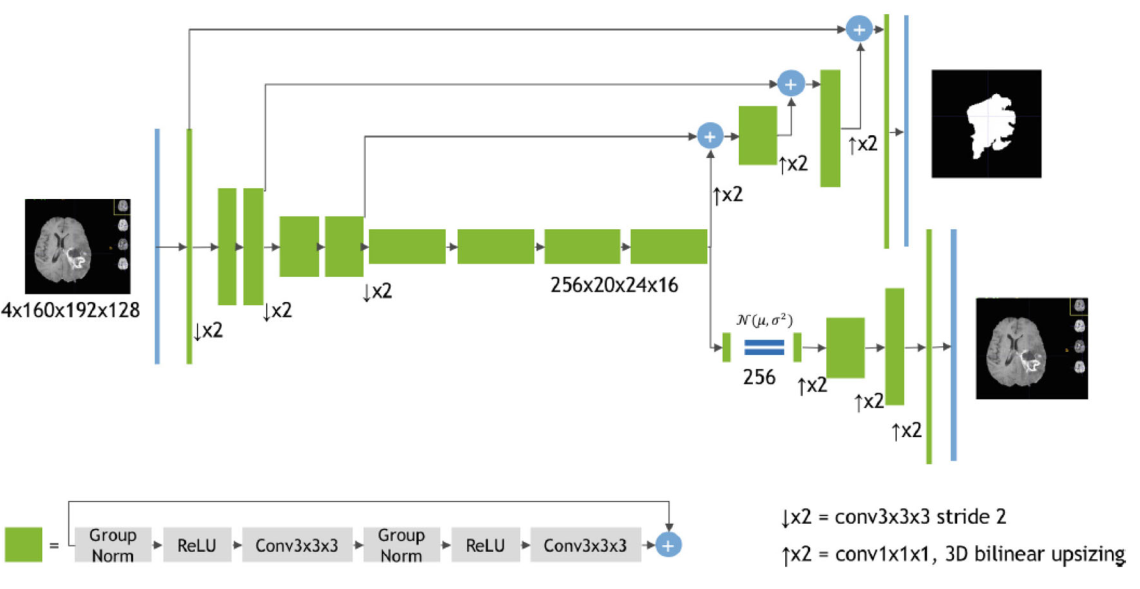
\includegraphics[width=1.0\linewidth]{imagenes/myroenko2019.png}
				\caption{Arquitectura del autoencoder regularizador de \cite{myronenko20193d}}
			\end{figure}
			
				
			\subsubsection{Funciones de pérdida especializadas}
			
			De forma más detallada, el problema del desbalanceo entre los diferentes tejidos se manifiesta durante el proceso de entrenamiento, en un gradiente excesivamente influenciado por los tejidos mayoritarios. Por ello, atacando directamente al problema multitud de trabajos proponen funciones de pérdida especializadas.
			
			Funciones de pérdida estándar en este problema incluyen categorical cross-entropy, cross-entropy y dice loss $D_{L}$.
			
			Una de las aproximaciones es el uso de utilizar una función de pérdida balanceada. Por ejemplo, añadir una penalización en función de la presencia del tejido segmentado para mitigar su escasa presencia respecto el total.
			
			Otro enfoque se basa en la combinación de diferentes funciones de pérdida en una nueva. Por ejemplo, una nueva función de pérdida de cross-entropy a nivel de píxel y dice loss podría ser su media.
			
			En general, funciones de pérdida que eviten el desbalanceo y mejoren el nivel de atención de las arquitecturas es beneficioso a todo tipo de problemas. Por ello, a diferencia de seguir funciones clásicas como cross-entropy, \cite{lin2017focal} proponen una nueva función llamada \textbf{Focal Loss} que será vista en años recientes en combinación con Dice Loss para diversos problemas de segmentación.
			
			
		\subsection{Métodos que tratan la información multi-modal}
		
		Las imágenes asociadas a una resonancia contienen diferentes tipos de imagen según las características de la frecuencia y contraste suministrado al paciente en su toma. Esta forma de proceder en la toma de resonancias es debido a las limitaciones de las imágenes IRM de poder representar y al menos para el ojo humano visualizar todos los tejidos importantes en el diagnóstico. Por ello, surge como idea clave tener métodos que tengan los objetivos de poder fusionar, relacionar y incluso distinguir en importancia las diferentes modalidades de imagen.
		
		Otras arquitecturas basadas en autoencoders como \cite{myronenko20193d} únicamente fusionan las cuatro modalidades como los canales de una imagen para un mismo slice concatenando las cuatro pruebas en la misma entrada, obteniendo entradas de dimensiones $ H \times W \times 4 $ en caso de 2D y $ H \times W \times D \times 4$ en caso de 3D.
		
		Sin embargo, usar concatenación o adición como método de fusión de los cuatro métodos no permitiría a la red de una forma directa aprender semánticamente la relación entre ellas. Por ello, en trabajos recientes se han adoptado mecanismos de atención aplicados a hacer aprender a la red de forma más robusta las diferentes modalidades e información espacial.
		
		\cite{zhou2021latent} proponen también una arquitectura encoder-decoder con la particularidad de crear un encoder y decoder especifico para cada una de las cuatro posibles representaciones, teniendo un espacio latente donde se fusiona la información de salida de los cuatro encoder dando un tratamiento especial a la fusión de las diferentes pruebas.
		
		A continuación, podemos ver la arquitectura especifica usada.
		
		\begin{figure}[H]
			\centering
			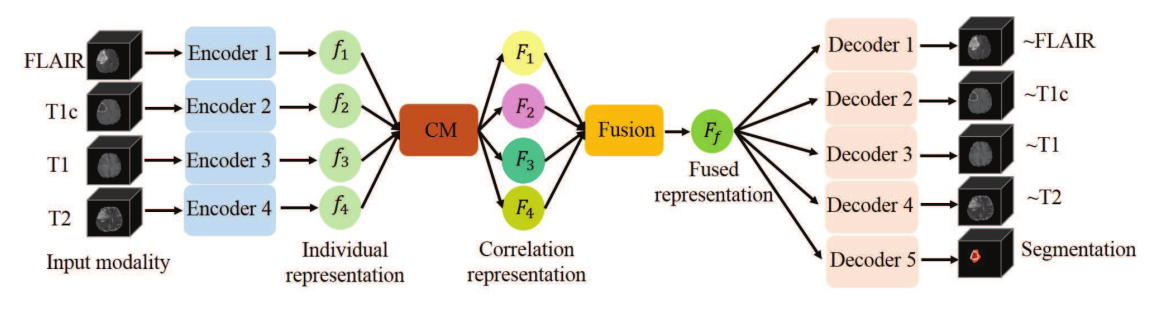
\includegraphics[width=0.75\linewidth]{imagenes/latentcorrelationrepresentation.png}
			\caption{Arquitectura de \cite{zhou2021latent}}
		\end{figure}
		
		Por un lado, transforma las representaciones individuales a representaciones correlacionadas. A través de lo que denominan \textbf{correlation model}.
		
		\begin{figure}[H]
			\centering
			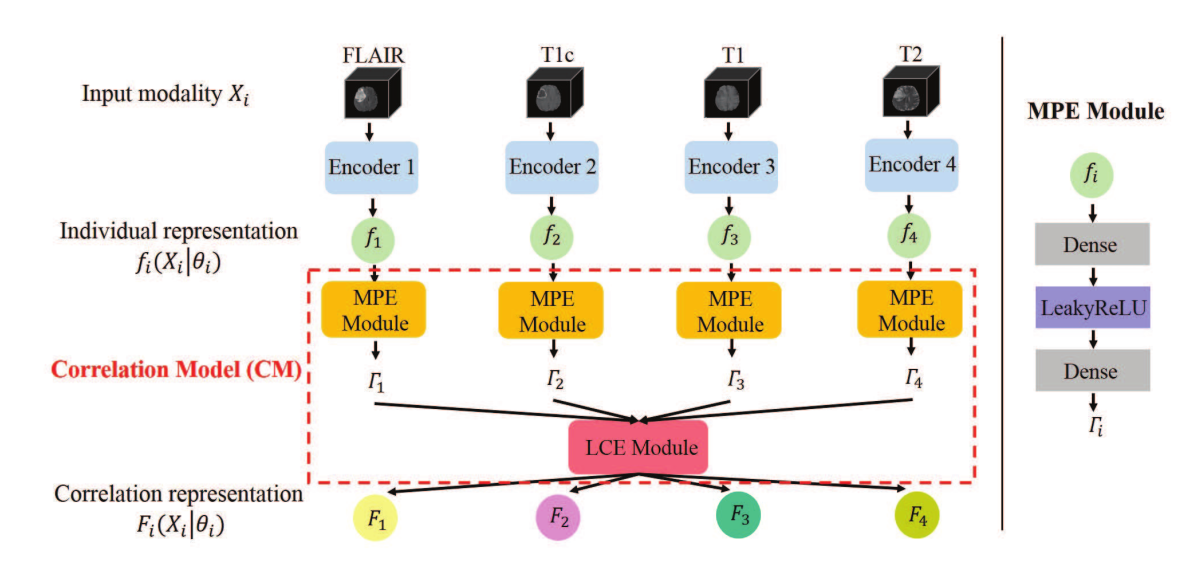
\includegraphics[width=0.75\linewidth]{imagenes/zhoufusionmodel.png}
			\caption{Modelo especializado en la correlación de las modalidades}
		\end{figure}
		
		El \textbf{correlation model} se compone de dos partes: módulo de estimación de parámetros (MPE) y un módulo de expresión de correlación lineal (LCE).
		
		El módulo de estimación de parámetros se compone de una de dos redes totalmente conectadas que vinculan cada representación salida de cada encoder con unos parámetros $ \Gamma_i = \{ \alpha_i , \beta_i , \gamma_i , \delta_i \}$
		
		El módulo de expresión de la correlación lineal (LCE) utiliza estos parámetros para obtener una versión correlacionada de cada representación individual aplicando: 
		$$ F_i (X_i | \theta_i ) = \alpha_i \odot \gamma_i f_j (X_j | \theta_j ) + \beta_i \odot f_k (X_k | \theta_k ) + \gamma_i \odot f_m (X_m | \theta_m ) + \delta_i , \quad (i \neq j \neq k \neq m)$$
		
		Tras ello, se fusiona las representaciones correlacionadas resultado. Permitiendo al modelo manejar de forma explícita la información multi-modal y dándole robustez ante pruebas faltantes. 
		
		\begin{figure}[H]
			\centering
			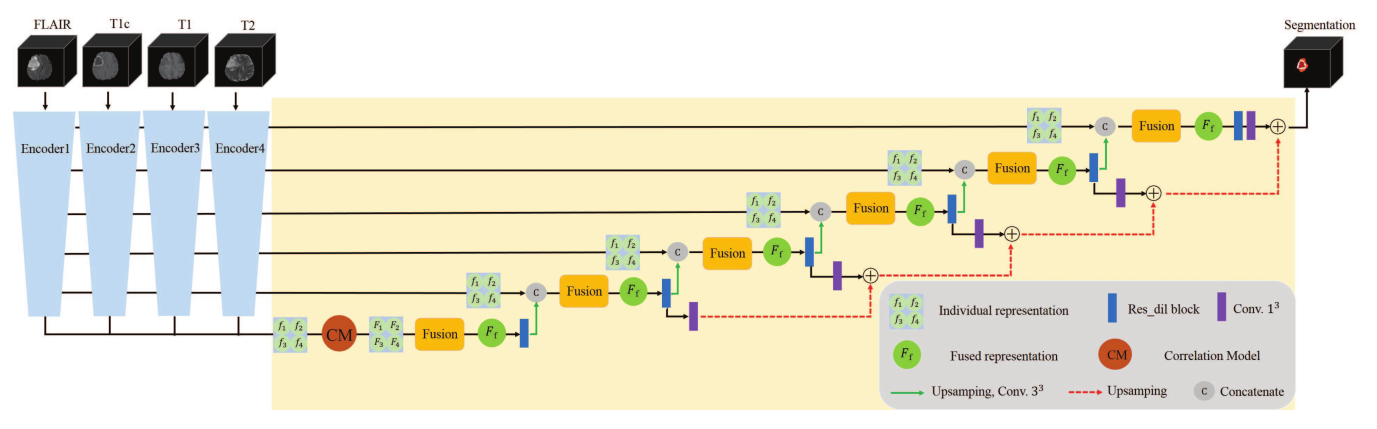
\includegraphics[width=1.1\linewidth]{imagenes/zhouarchitecture.png}
			\caption{Red \cite{zhou2021latent} de fusión de representaciones latentes}
		\end{figure}
		
		Si bien esta arquitectura da ligeramente peores resultados que \cite{myronenko20193d} define un paso más en el estado del arte al usar menos recursos computacionales.


\section{Nuevas enfoques para la segmentación}

	Las soluciones más relevantes presentadas en la revisión histórica que se ha hecho anteriormente se basan en la aplicación de la convolución sobre las imágenes de resonancia magnética. En el diagnóstico de tumores cerebrales ha tenido largo recorrido el uso de redes neuronales convolucionales. 
	
	Con la inclusión de las arquitecturas transformadoras se planteó un nuevo modelo que podía traer ventajas significativas. No siendo la imagen médica y en concreto este problema una excepción.
	
	Con la adaptación de los transformers al campo de la visión, los Vision Transformers podría ser un modelo más unificador, paralelizable y que ofreciera mejores resultados que las redes convolucionales al romper con la localidad que supone el uso de convoluciones. 
	
	En las soluciones más recientes de la segmentación de tumores cerebrales se introduce el uso de Vision Transformers con estas expectativas.
	
	\subsection{Basados en Transformers}
	
	A continuación, se presentan las soluciones principales que hacen uso de una arquitectura basada en Transformers para la segmentación de tumores cerebrales.
	
	\subsubsection{}
	
	\subsection{Basados en aprendizaje no supervisado}
